\documentclass[11pt,a4paper]{article}

% ---------- layout and fonts ----------
\usepackage[margin=2.4cm,top=2.2cm,bottom=2.4cm]{geometry}
\usepackage[utf8]{inputenc}
\usepackage{microtype}
\usepackage{amsmath}
\usepackage{graphicx}
\usepackage{booktabs}
\usepackage{tabularx}
\usepackage{float}
\usepackage[font=small,labelfont=bf,labelsep=period,skip=6pt]{caption}
\usepackage{enumitem}
\usepackage{titlesec}
\usepackage{fancyhdr}
\usepackage[hidelinks]{hyperref}

\graphicspath{{figures/}}
\setlist{nosep,leftmargin=1.4em,topsep=3pt}
\setlength{\parskip}{4pt}
\setlength{\parindent}{0pt}

\titleformat{\section}{\Large\bfseries}{\thesection}{0.6em}{}
\titleformat{\subsection}{\large\bfseries}{\thesubsection}{0.6em}{}
\titlespacing*{\section}{0pt}{14pt}{6pt}
\titlespacing*{\subsection}{0pt}{10pt}{4pt}

\pagestyle{fancy}
\fancyhf{}
\renewcommand{\headrulewidth}{0pt}
\fancyfoot[L]{\small DAYFIT --- EECE 490 final report}
\fancyfoot[R]{\small\thepage}

\begin{document}

% ---------- title block ----------
\begin{center}
{\bfseries\fontsize{20}{24}\selectfont DAYFIT: Finding Similar Garments}\\[4pt]
{\normalsize Mouhammed Soumaille}\\[2pt]
{\normalsize EECE 490 Machine Learning, American University of Beirut, Fall 2026}\\[2pt]
{\small Code, results and lab notebook: \url{https://github.com/mouhammed-soumaille/dayfit}}
\end{center}

\begin{abstract}
\noindent Shoppers often see a garment they want but cannot describe it well enough to find it in an online
shop, and large shops lose those sales because text search and menus only work when the shopper can name what
they saw. DAYFIT lets the shopper search with the photo instead: it returns the five most similar items from
the shop's catalogue, labelled with the garment type and colour it measured. The search uses FashionSigLIP
image embeddings, fine-tuned on the catalogue with synthetic phone photos. On 481 held-out real street photos
(LookBench), the photo search puts the exact item first for 50\% of photos, four times as often as a
classical image search (12\%) and clearly ahead of a short typed search (31\%); only an idealised shopper who
types every attribute in the shop's own words matches it (49\%). Whether the shopper marks the garment or
sends the whole photo matters more than fine-tuning (50\% vs 39\%), while fine-tuning mainly buys robustness
to blur (+6 to +21 points). In a final test fixed in advance, on 83 photos of my own wardrobe, the system as
deployed returned the right kind of garment in its top 5 for 98.5\% of photos, but the exact article type
for only 75\%. A learned re-ranker and the system's ``not sure'' message did not work. The system runs as a
FastAPI service with a web page over a 54,178-item catalogue, answers in 266\,ms on a 4-core CPU and never
stores the photos.
\end{abstract}

%=====================================================================
\section{The problem}

\textbf{Who it is for.} DAYFIT has two users.
\begin{itemize}
\item \textbf{The shopper}, who has seen a garment (on someone in the street, in a photo, in a shop window)
  and wants it, or something like it.
\item \textbf{The store}, in particular one with a large catalogue. A shop with tens of thousands of items
  cannot expect shoppers to browse them, and every search that comes back empty is a lost sale. ``Search by
  photo'' gives shoppers a way in when they cannot find the words. DAYFIT would run as such a feature on one
  shop's website, so it only suggests what that shop sells. The demo catalogue has 54,178 items, the scale
  where browsing by menu stops being practical.
\end{itemize}

\textbf{How it is done today.} On a shop's site, shoppers type words (``brown knit sweater'') or click
through menus (type, colour) and scroll. Both need the shopper to \emph{name} what they saw, which is exactly
what is hard: was it khaki or olive, a bomber or a field jacket? The bigger the catalogue, the more items share
the same few words. Outside the shop, general tools such as Google Lens search the whole web rather than one
shop's stock. I compare DAYFIT against keyword search, menu filters and a classical (non-deep-learning)
image search. I did not compare against Google Lens.

\textbf{The two questions I measure.}
\begin{itemize}
\item \textbf{Right kind of garment} (``show me things like this''): is the garment group (tops, bottoms,
  outerwear, footwear, \dots) right in the top 5 results? This was the main metric of the approved proposal,
  with a target of 0.90. I call it \emph{group P@5}.
\item \textbf{Exact item first} (``is this the very item?''): is the photographed item the first result?
  This is \emph{R@1}. I added it because the first question turned out to be too easy for the alternatives:
  a typed category already gets 0.98 and a menu gets 1.0 by construction, so group P@5 alone cannot show that
  a photo adds anything. R@1 can.
\end{itemize}

\textbf{The constraints} (from the proposal): it must work on imperfect phone photos, and it must answer fast
enough to feel immediate. I set a budget of 500\,ms of server time per search on a 4-core CPU.

%=====================================================================
\section{Related work}

Matching a street photo of a garment to the same product in a shop was posed as a research problem by
Kiapour et al.~\cite{kiapour2015}. LookBench~\cite{lookbench} is a recent benchmark built from current
street-style photos and live shop catalogues; I use its real street-photo subset as my main test. DAYFIT
starts from Marqo's FashionSigLIP~\cite{marqo2024}, an image--text model adapted to fashion products, and
fine-tunes it on the shop's catalogue. DAYFIT does not propose a new model; its contribution is a careful
evaluation of such a model as a shop feature, against the alternatives a shopper actually has, on real
photos, and in a final test fixed in advance.

%=====================================================================
\section{How DAYFIT works}

\begin{figure}[!htbp]
\centering
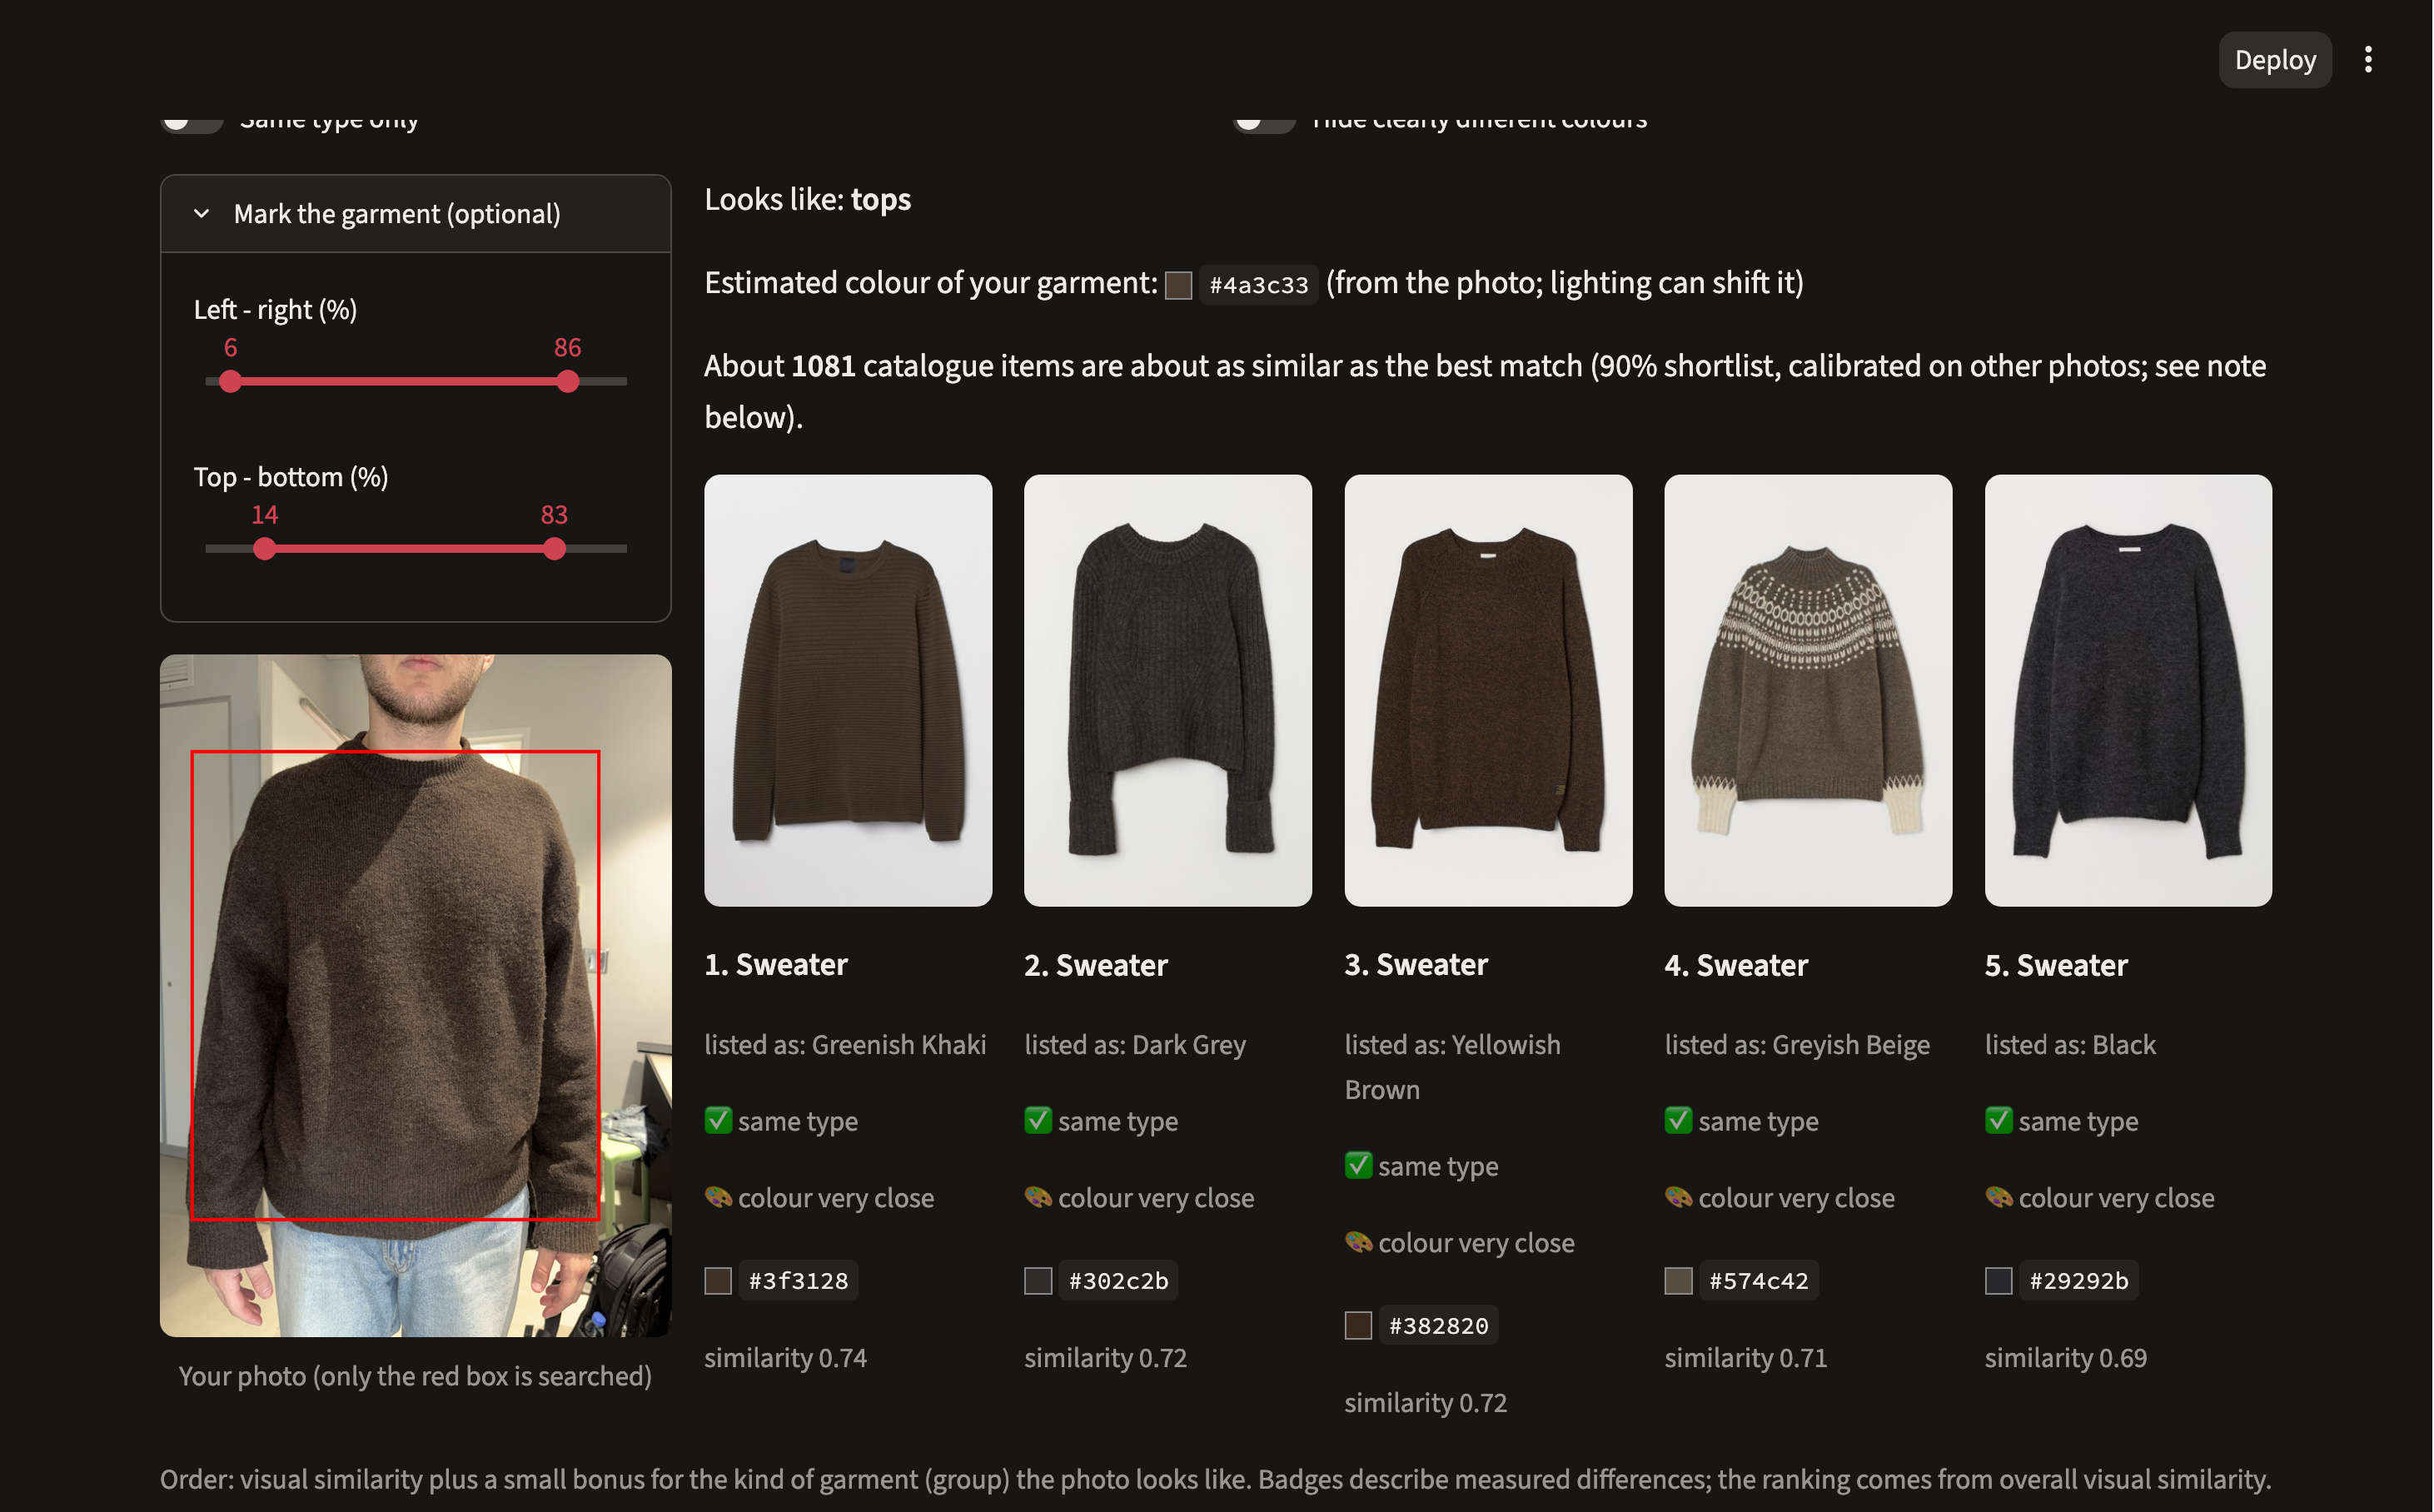
\includegraphics[width=\textwidth]{demo_sweater_crop.png}
\caption{The app on a photo of my own sweater, which is not in the catalogue. Only the red box is searched.
The five results are similar brown knit sweaters, each with a type badge and a colour badge.}
\end{figure}

\textbf{The model.} Each photo and each catalogue image is turned into a vector (an \emph{embedding}) by
FashionSigLIP, a vision model pretrained on fashion images. The search returns the catalogue items whose
vectors are closest to the photo's (cosine similarity). I fine-tuned the model on the catalogue: each
catalogue image was paired with a synthetic ``phone photo'' of itself (random background, rotation, crop,
lighting, blur, JPEG), and the model learned to put each pair close together and other items apart
(contrastive training, 5 epochs, last 4 of 12 blocks). Training with random batches beat training with
batches of same-type items, which made the model worse at telling garment types apart.

\textbf{Ranking.} The order is the similarity plus a small bonus, $0.05 \times P(\text{item's group}\mid
\text{photo})$, from a second, zero-shot model that guesses the garment group. Kids' items are hidden and
duplicate product photos are shown once.

\textbf{What the page shows.} The five results; a \emph{type badge} (shown only when the group guess is at
least 90\% confident); a \emph{colour badge} comparing the garment's estimated colour with each result; an
out-of-catalogue warning (``this looks like a skirt; our catalogue has no skirts''); two optional filters
(same type only, hide clearly different colours) that hide results without changing the order; and an
optional crop box to mark the garment. The badges describe measured differences, not the model's reasons.

\textbf{Two catalogues.} All experiments use an evaluation catalogue of 6,197 items (Kaggle Fashion Product
Images~\cite{fpi}, 14 types). The demo uses a bigger app catalogue of \textbf{54,178} items (68 types): more items from
the same dataset plus 21,037 newer H\&M products~\cite{hm}, so it looks more like a real shop.

%=====================================================================
\section{How I tested it}

\textbf{Three kinds of test photo.}
\begin{enumerate}
\item \textbf{Synthetic phone photos} of catalogue items (294 items). Useful early on, but the fine-tuned
  model was trained on the same kind of synthetic photo, so these mostly measure how well it learned that
  augmentation (fine-tuning gains +15.6 points here, about +2 on real photos). They are a secondary result
  and not used below.
\item \textbf{Real street photos} from the LookBench benchmark~\cite{lookbench}: 981 photos of people wearing items from a
  3,278-item shop, searched against an official corpus of 61,553 images (the shop items plus 58,275
  distractors). I split them once into a development half (500) and a test half (481), keeping photos of
  the same street picture or item on one side. Every method was tuned on the development half and run
  \emph{once} on the test half.
\item \textbf{My own wardrobe} (the final test, ``D9''): one phone photo of each garment I own, taken after
  the rules, the model and my expected result were written down, and run exactly once.
\end{enumerate}

\textbf{Is a difference real?} Every number comes with a 95\% confidence interval from a bootstrap (resample
the photos 2,000 times and see how much the number moves). Comparisons between two methods are paired (same
photos) and resample groups of related photos together; when several methods are compared at once, the
p-values are corrected for multiple tests (Holm).

\textbf{What the test half can and cannot show.} I chose the app's model (fine-tuned with random batches, over the pretrained model and an ensemble) using
\emph{all} 981 LookBench photos, before I froze the development/test split. So the test half is clean for
everything decided afterwards (the ranking bonus, the re-ranker, the baselines), but not for the choice of
the model itself: the fine-tuned vs pretrained comparison is slightly optimistic. The own-wardrobe test is
the check that was never touched.

%=====================================================================
\section{Results}

\subsection{A photo against the alternatives}

\begin{figure}[!htbp]
\centering
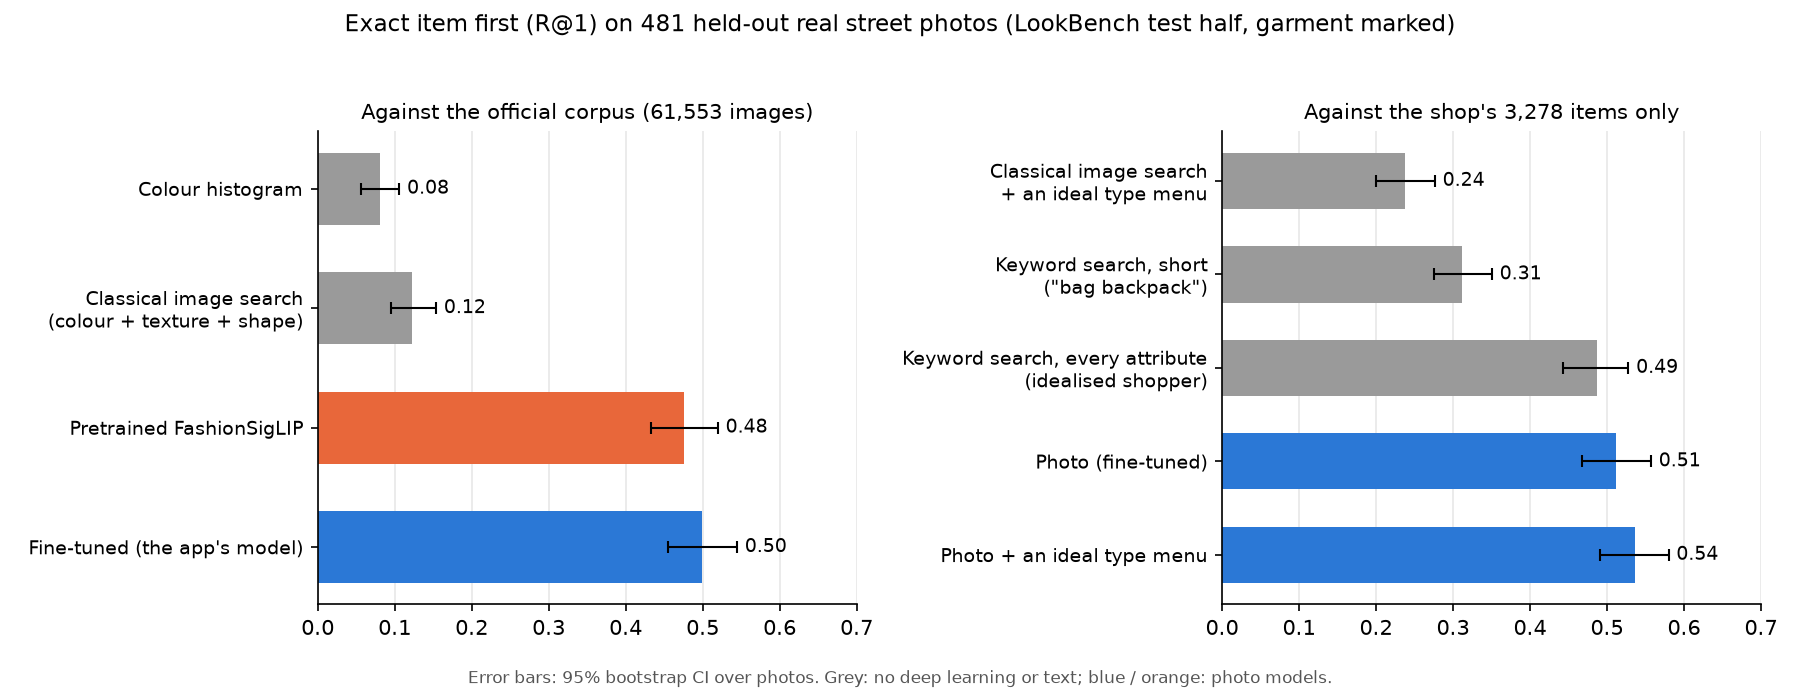
\includegraphics[width=\textwidth]{fig15_headline_real.png}
\caption{Exact item first on the 481 test photos, with 95\% confidence intervals. Left: searching the
official 61,553-image corpus. Right: searching only the shop's 3,278 items, which is needed for anything that
uses item text or type labels (keyword search, menus).}
\label{fig:headline}
\end{figure}

\begin{table}[H]
\centering\small
\begin{tabularx}{\textwidth}{Xcc}
\toprule
\textbf{Method} (shop's 3,278 items, test half) & \textbf{Exact item first} & \textbf{Right kind of garment} \\
\midrule
Classical image search + an ideal type menu & 0.237 & 1.0 (by construction) \\
Keyword search, short (``bag backpack'') & 0.312 & 0.983 \\
Keyword search, every attribute in the shop's words (idealised) & 0.486 & 0.986 \\
\textbf{Photo, fine-tuned model} & \textbf{0.511} & 0.871 \\
Photo + an ideal type menu & 0.536 & 1.0 (by construction) \\
Photo + group bonus (\emph{the app's ranking}) & 0.509 & \textbf{0.905} \\
\bottomrule
\end{tabularx}
\caption{The same comparison with both metrics. On the official corpus the fine-tuned model reaches 0.499
exact-item-first and 0.688 exact-item-in-top-5; the colour histogram 0.081 and the classical search 0.123.}
\end{table}

\textbf{What this shows.}
\begin{itemize}
\item \textbf{The photo wins wherever the shopper can't describe the garment perfectly.} It finds the exact
  item first four times as often as a classical image search (0.50 vs 0.12) and clearly more often than a
  short typed search (0.51 vs 0.31). Only a shopper who types every attribute in the shop's own words ties it
  (0.49 vs 0.51, no significant difference). That shopper doesn't exist; the honest pitch is that \emph{a
  photo matches a perfect description without anyone having to write one}.
\item \textbf{For ``the right kind of garment'', a menu is unbeatable.} The photo alone gets it right for
  0.87 of photos; a menu always does. The app's group bonus raises the photo to \textbf{0.905}, meeting the
  proposal's 0.90 target on held-out photos, at no cost in exact-item accuracy (0.509 vs 0.511, not
  significant).
\item \textbf{A 19 times bigger corpus costs only about 2 points}: the 58,275 distractors rarely beat the true
  item.
\end{itemize}

\subsection{What matters for a real shopper's photo}

LookBench photos are hand-drawn crops of the garment, but the app sends the \emph{whole} photo unless the
shopper marks the garment. That turns out to matter more than any model change I tried.

\begin{figure}[!htbp]
\centering
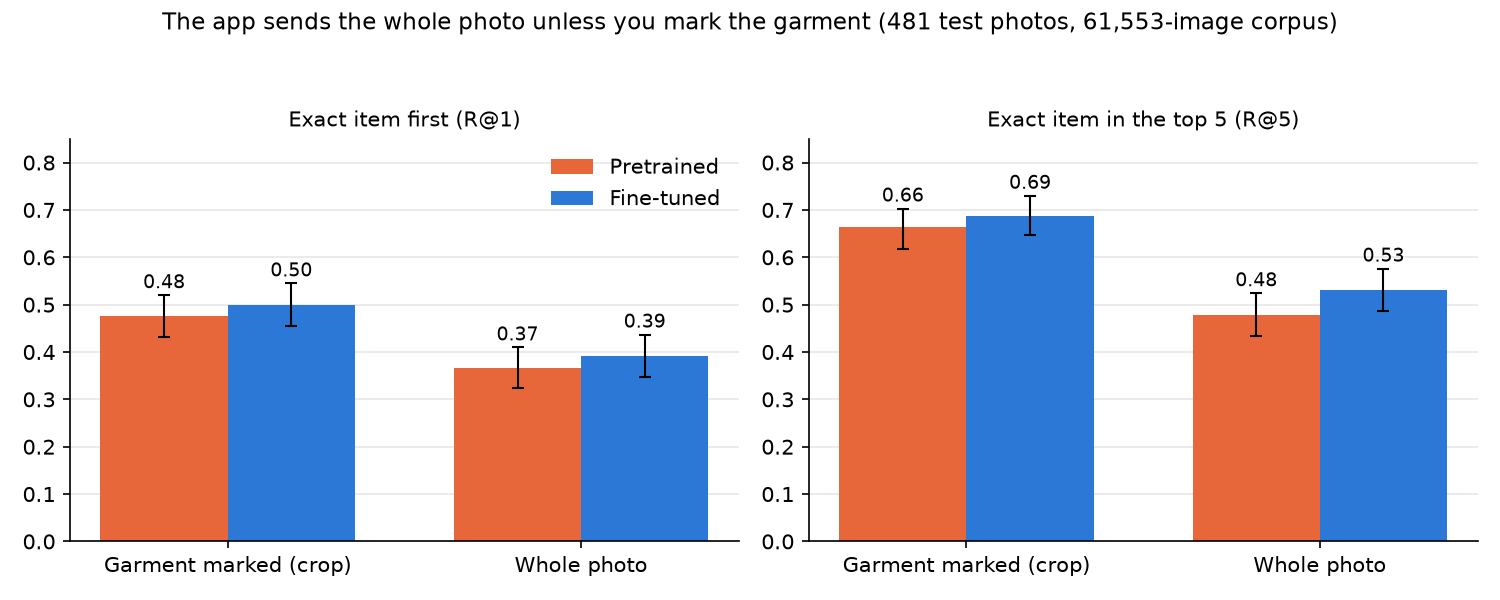
\includegraphics[width=0.92\textwidth]{fig16_crop_vs_whole.png}
\caption{Garment marked vs whole photo (test half, official corpus). Marking the garment adds about 11 points;
fine-tuning adds about 2--3.}
\end{figure}

Exact item first drops from \textbf{0.50} to \textbf{0.39} with the whole photo, and ``right kind of garment''
drops from 0.87 to 0.68. So the app now recommends marking the garment, and the 0.905 above should be read as
a number for marked garments.

\textbf{Bad photos.} I applied fixed filters (blur, motion blur, darkness, black-and-white, coloured light) to
all 981 real crops. This is where fine-tuning earns its place: on blurred photos it adds \textbf{+6 to +21
points} over the pretrained model, including motion blur, which it never saw in training. For colour
changes it never saw, it adds nothing beyond its clean-photo gain. Very strong blur breaks every model (exact
item first 0.12).

\begin{figure}[!htbp]
\centering
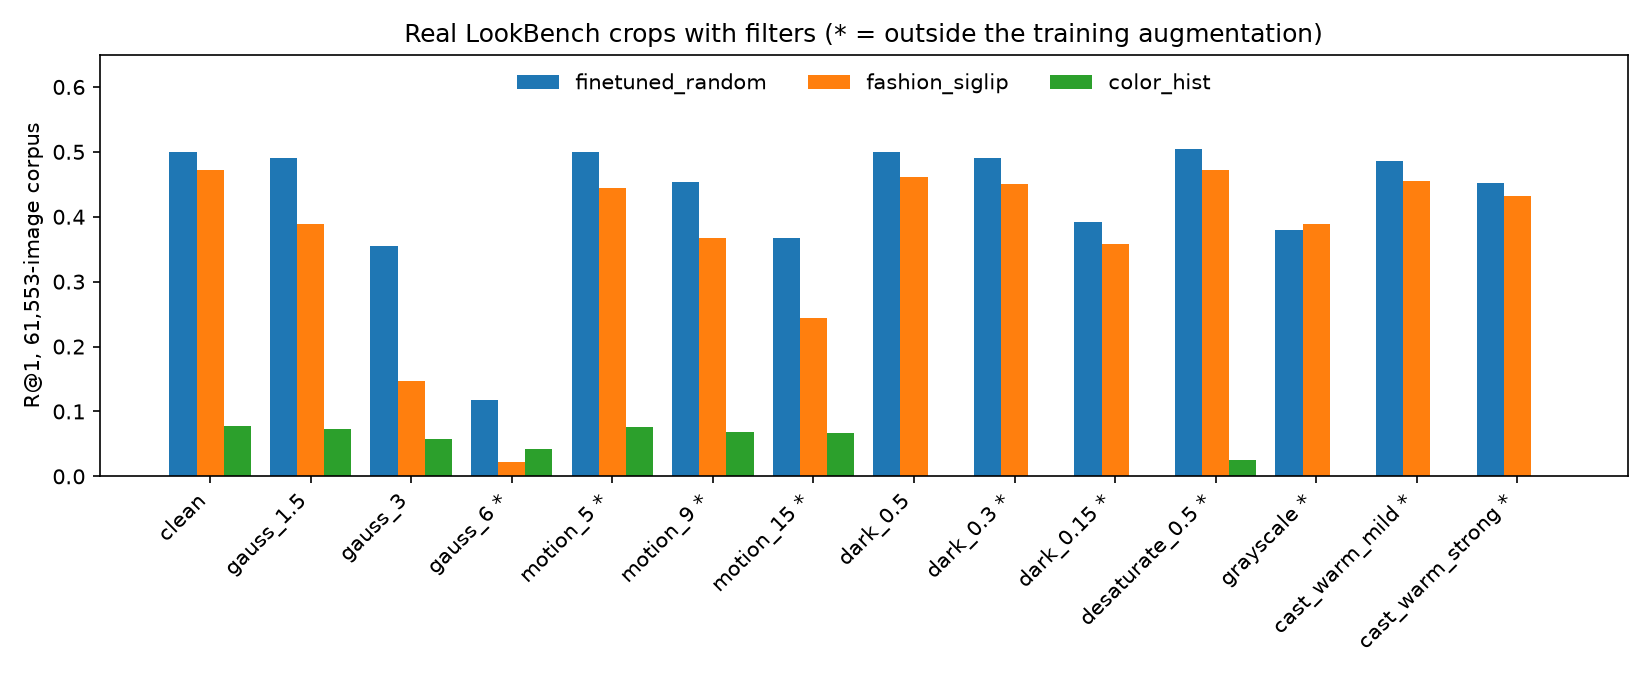
\includegraphics[width=0.92\textwidth]{robustness.png}
\caption{Exact item first under each filter (all 981 real crops; * = a filter outside the training
augmentation).}
\end{figure}

On clean photos, the fine-tuning gain is small: +2.3 points on the test half, which is \emph{not}
statistically significant ($p = 0.07$). On whole photos it is +2.5 points ($p = 0.04$).

\subsection{The final test: my own wardrobe}

I photographed every garment I own, one photo each, in one session with my phone, with no editing and no
crop box (83 photos: 39 t-shirts, 9 sweaters, 2 hoodies, a shirt, 14 bottoms, 6 jackets and a blazer, 4 pairs
of shoes, 7 accessories, a wallet). Before taking any photo I wrote down the rules, froze the model and
predicted the result: between 0.70 and 0.90. Each photo was labelled by hand and checked before a single run
against the 54,178-item app catalogue, exactly as the app is shipped.

\begin{table}[H]
\centering\small
\begin{tabularx}{\textwidth}{Xcc}
\toprule
\textbf{Result} & \textbf{Value [95\% CI]} & \textbf{Photos} \\
\midrule
\textbf{The app as shipped}: right kind of garment in the top 5 & \textbf{0.985} [0.968, 0.998] & 82 \\
Fine-tuned model: same article type in the top 5 (evaluation catalogue) & 0.745 [0.668, 0.822] & 65 \\
Pretrained FashionSigLIP, same & 0.711 & 65 \\
Colour histogram, same & 0.092 & 65 \\
\bottomrule
\end{tabularx}
\caption{The own-wardrobe test (run once). The wallet is excluded from the first row (the shop sells no
wallets); the second row uses only photos whose type is one of the 14 evaluation types.}
\end{table}

\begin{figure}[!htbp]
\centering
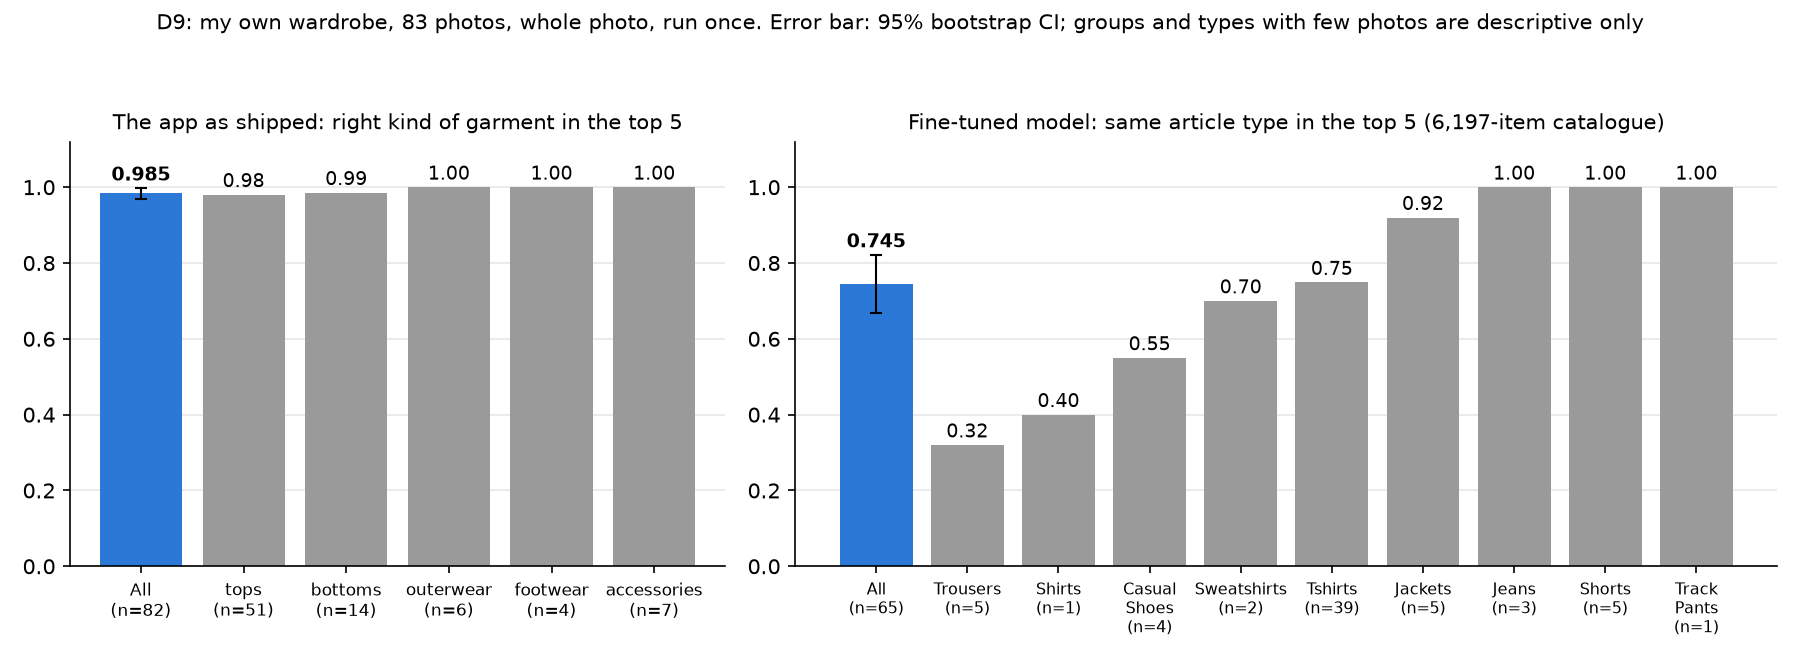
\includegraphics[width=\textwidth]{fig17_d9.png}
\caption{Left: the app, per garment group. Right: the fine-tuned model, per article type. Groups and types
with few photos are descriptive only.}
\end{figure}

\begin{figure}[!htbp]
\centering
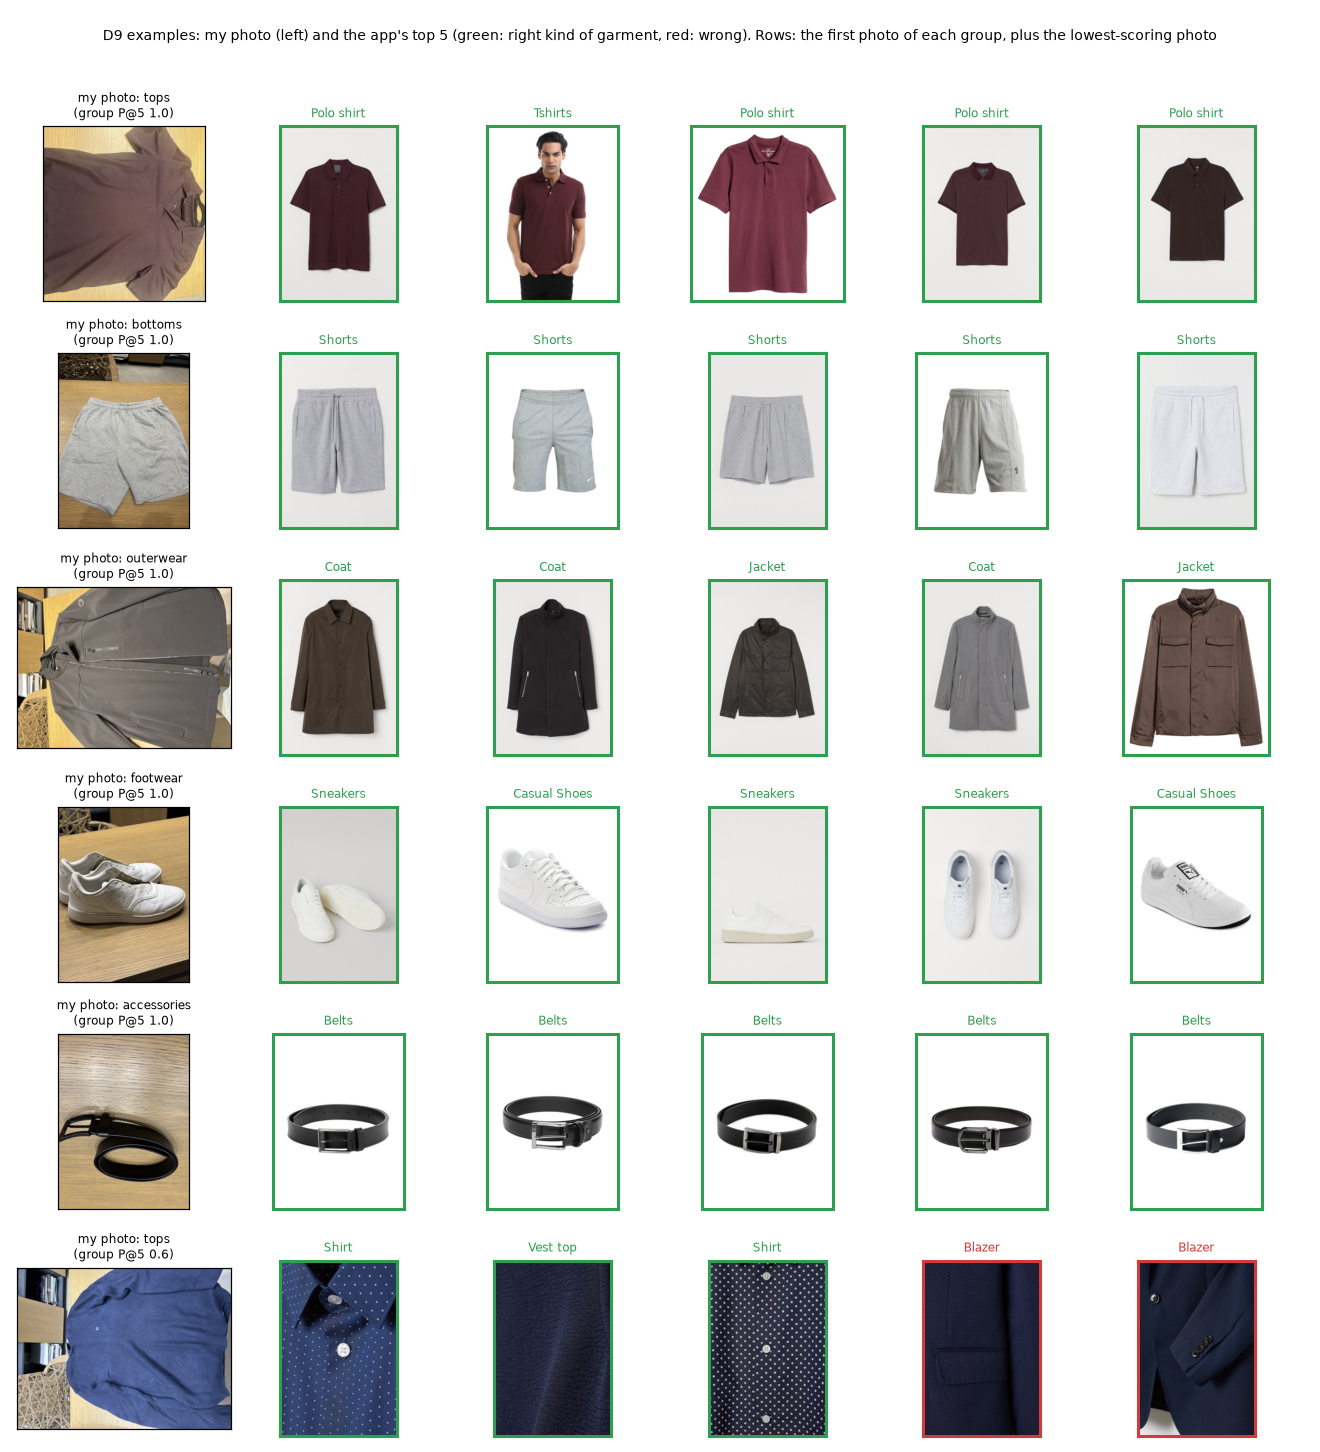
\includegraphics[width=0.95\textwidth]{fig18_d9_gallery.png}
\caption{Examples, chosen by a fixed rule rather than by looking: the first photo of each group, and the
lowest-scoring photo. Green: right kind of garment; red: wrong.}
\end{figure}

\textbf{What this shows.}
\begin{itemize}
\item \textbf{Better than I predicted, because these photos are the easy case.} A garment laid flat or on a
  hanger looks a lot like a shop's product photo. This does not contradict the street-photo numbers: a
  shopper photographing a stranger's jacket is closer to the whole-photo result (0.68).
\item \textbf{The type is harder than the group.} Jeans, shorts and jackets are almost always right;
  trousers come back as track pants (0.32) and casual shoes as sports shoes (0.55). Right group, wrong type.
\item \textbf{The badges and the warning worked}: the group badge appeared for 92\% of photos and was right
  every time; the out-of-catalogue warning fired once, on the wallet, and never on the 82 garments the shop
  sells.
\end{itemize}

\textbf{A mistake I found after the run.} One photo, labelled as a t-shirt, turned out to be a photo of my
finger, taken by accident. The rules say nothing is dropped after seeing results, so the table keeps it.
Without it the two main numbers are 0.990 and 0.756; no conclusion changes.

\subsection{What did not work}

\begin{itemize}
\item \textbf{A learned re-ranker.} I trained a gradient-boosted model on 500 labelled street photos to
  re-order the top 20 using nine features (similarities from three models, small-patch matching, colour,
  type agreement). It gains +2.1 points of exact-item-first, which is not significant ($p = 0.12$). Adding
  1,011 studio photos did not help. Mixing in a second model (DINOv2) or colour similarity did not help
  either.
\item \textbf{The ``not sure'' message.} It was calibrated on LookBench, whose similarity scores differ from
  the app catalogue's. On my wardrobe it fired on 47\% of photos, and the results were just as good when it
  fired as when it didn't (0.984 vs 0.986). In the app it is too cautious to be useful.
\item \textbf{The ``shortlist size''} (how many items are about as similar as the best match, with a 90\%
  guarantee) works on LookBench but is far too long in the app (median 1,552 items), so the page hides it.
\end{itemize}

%=====================================================================
\section{Where it fails}

\textbf{Right kind, wrong design.} On the development half, 87\% of the misses already have the right kind
of garment first: the model finds \emph{a} black leather jacket with a shearling collar, not \emph{that}
jacket. In 97 of the 236 misses the true item is not even in the top 20, so no re-ranking can fix them; that
needs a better model, for example one trained on real street-to-shop photo pairs.

\begin{figure}[!htbp]
\centering
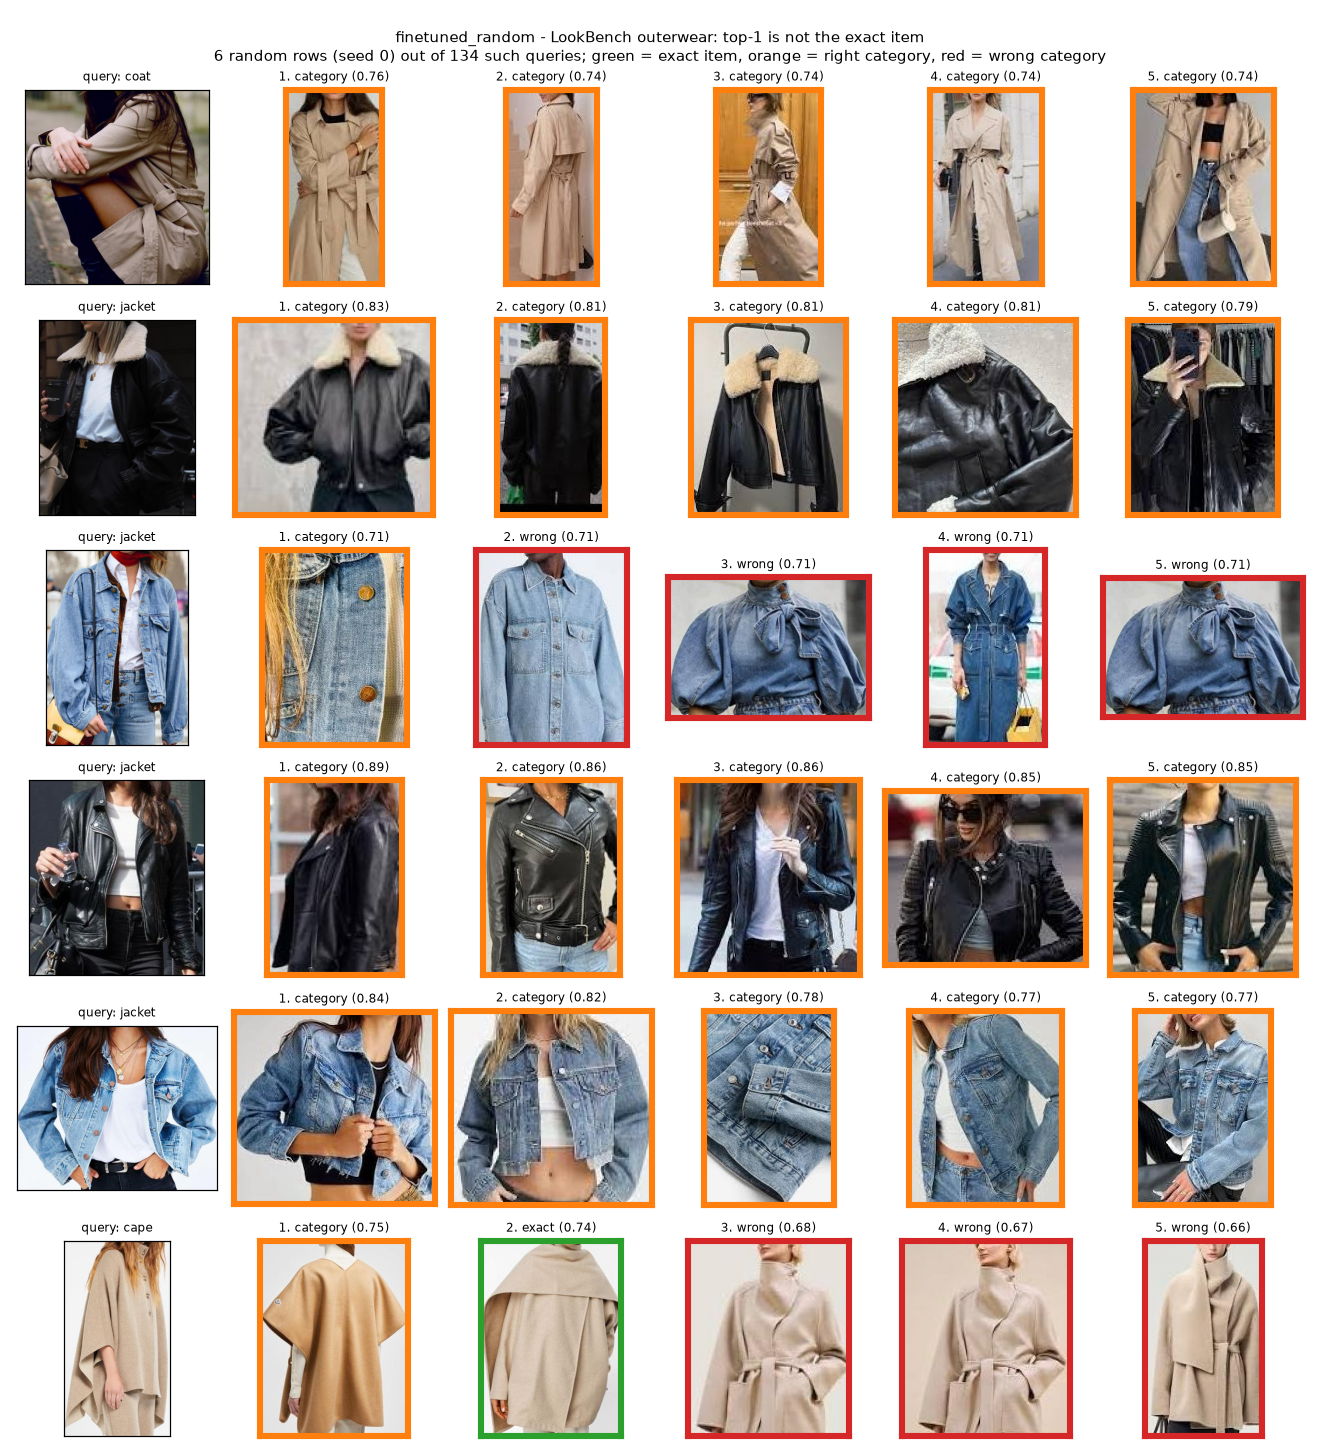
\includegraphics[width=0.95\textwidth]{fig10_failures_real_outerwear.png}
\caption{Six random outerwear photos whose first result is not the exact item (orange: right category, red:
wrong category, green: the exact item). The results are near-identical coats and jackets.}
\end{figure}

\textbf{It doesn't know when a photo isn't clothing.} The accidental finger photo got back blazers, shirts
and a scarf, with no ``not sure'' and no warning: the out-of-catalogue check only knows clothing the shop
doesn't sell. A photo of a cup or a dog would get five garments too.

\textbf{Other failure modes:} very blurry photos (and ``not sure'' catches only 19\% of them); very dark
photos, which often get a wrong ``different colour'' badge; and a colour estimate that can pick up the
background when the whole photo is sent.

%=====================================================================
\section{The system}

\textbf{Architecture.} A FastAPI service loads the model and the 54,178 catalogue embeddings once, then
answers \texttt{POST /search} with the results, badges, warnings and the search time. A Streamlit page calls
the API. Both run with one command in Docker (\texttt{docker compose up}); the page waits until the API
reports healthy. The app's code is separate from the experiment code: the Docker image contains no evaluation
code, and the app builds its model with the same function the experiments use, so it searches exactly like
the evaluated model (checked: identical top-5 results and scores on saved test queries).

\textbf{Speed.} Median \textbf{266\,ms} per search in Docker on 4 CPU cores, inside the 500\,ms budget;
129\,ms on a laptop CPU and 36\,ms on the laptop GPU. The second (type) model is 56\,ms of that and can be
switched off on slow machines.

\textbf{Privacy by construction.} Uploaded photos are read straight into memory and never written to disk or
logged. A test checks that a search writes no file, and in Docker the API runs on a read-only file system.

%=====================================================================
\section{Responsible use and limitations}

\textbf{When not to use it.}
\begin{itemize}
\item \textbf{Not as a promise of the exact item.} The exact item comes first about half the time on marked
  garments and 39\% on whole photos. Results should be presented as ``similar items'', not as ``this is your
  item''.
\item \textbf{Not on photos of people who didn't agree to it.} The app stores nothing, but a ``search by
  photo'' feature invites photos of strangers. A real deployment should tell shoppers to photograph garments,
  not people.
\item \textbf{Not commercially with these images.} Fashion Product Images, LookBench and the H\&M data are for
  non-commercial research only.
\end{itemize}

\textbf{Limitations of the evidence.}
\begin{itemize}
\item One real-photo benchmark (LookBench), with confidence intervals of about $\pm$4--5 points, and a model
  chosen before its split was frozen.
\item The app as shipped was measured only on my own wardrobe: one person, one session, mostly tops, no
  dresses or bags, garments on a plain surface.
\item ``Similar'' is only measured as ``same kind of garment''. Whether the top 5 actually look alike was not
  judged by people.
\item \textbf{Catalogue bias.} The base catalogue (an Indian e-commerce site, 2011--12) leans towards men's
  and older styles; none of its jeans are wide-leg. Women's and current styles depend mostly on the H\&M
  items, whose own type labels are noisy.
\item Kids' items are hidden, not detected: a photo of a kids' garment gets the most similar adult items.
\end{itemize}

%=====================================================================
\section{Possible extensions}

\begin{itemize}
\item \textbf{A ``is this a garment?'' check.} A small classifier in front of the search, so that a photo of a
  finger, a cup or a dog is answered with ``this doesn't look like clothing'' instead of five garments.
\item \textbf{Automatic garment detection.} Marking the garment is the single biggest improvement I found
  (39\% to 50\% exact-item-first). A garment detector could draw the box automatically, or offer one box per
  garment when the photo shows a whole outfit.
\item \textbf{Training on real street-to-shop pairs.} Most misses are the right kind of garment with the
  wrong design, and in 41\% of them the true item is not even in the top 20. Training on pairs of real street
  photos and shop photos, rather than synthetic phone photos, is the most direct way to fix this.
\item \textbf{Recalibrating ``not sure'' on the store's own catalogue.} The message was calibrated on another
  catalogue and does not work in the app. A few hundred labelled searches on the store's catalogue would let
  it be calibrated where it is used.
\item \textbf{Measuring ``similar'' with people.} Asking shoppers whether the top 5 actually look like what
  they photographed would measure the case that matters most when the shop doesn't sell the exact item.
\item \textbf{Text and photo together.} Letting the shopper add a few words (``but in black'', ``longer'') to
  the photo, which models such as CLIP and SigLIP already support, since they embed text and images in the
  same space.
\item \textbf{Scaling to a store's full catalogue.} At hundreds of thousands of items, the exact search used
  now (comparing the photo with every item) would be replaced by an approximate nearest-neighbour index,
  with the catalogue embeddings updated as products are added.
\item \textbf{Learning from shopper feedback.} Once deployed, clicks and purchases give a reward signal.
  A contextual bandit, a simple form of reinforcement learning, could use it to tune the ranking (for example
  the weight of the group bonus) for each store, while occasionally exploring lower-ranked items. This needs
  care: shoppers click what is shown first, and a system that learns from its own clicks can reinforce its
  mistakes and over-promote popular items.
\item \textbf{A wider final test}, with other people's wardrobes (dresses, bags, skirts) and photos taken in
  the street rather than on a plain surface.
\end{itemize}

%=====================================================================
\section{Reproducibility and contributions}

The repository contains the code, every saved result table, the figures, the development/test split and a
lab notebook (\texttt{report/results\_log.md}) with every experiment's plan written \emph{before} it was run,
every result, and every correction and negative result. The README lists the commands to rebuild the
catalogues, train the model and reproduce each number; each script checks itself against a saved number and
stops if it does not match. The datasets, checkpoint and indexes are not in git (size and licences) and are
regenerated by those commands.

\textbf{Contributions.} I wrote the code with the help of Claude (an AI assistant) and reviewed all of its
outputs. The analysis is purely mine. The report was written by me with the help of Claude, which helped in some table rendering and finding the required references.

%=====================================================================
\begin{thebibliography}{99}\small
\bibitem{fpi} P.~Aggarwal. Fashion Product Images Dataset. Kaggle, 2019.
  \url{https://www.kaggle.com/datasets/paramaggarwal/fashion-product-images-dataset}
\bibitem{hm} H\&M Group. H\&M Personalized Fashion Recommendations. Kaggle competition dataset, 2022.
\bibitem{kiapour2015} M.~H.~Kiapour, X.~Han, S.~Lazebnik, A.~C.~Berg and T.~L.~Berg. Where to buy it:
  matching street clothing photos in online shops. \emph{ICCV}, 2015.
\bibitem{lookbench} C.~Gao, S.~Xue, Y.~Peng, J.~Fu, T.~Gu, S.~Li and F.~Zhou. LookBench: a live and holistic
  open benchmark for fashion image retrieval. arXiv:2601.14706, 2026.
\bibitem{marqo2024} Marqo. Marqo-FashionCLIP and Marqo-FashionSigLIP. Model cards, 2024.
  \url{https://huggingface.co/Marqo/marqo-fashionSigLIP}
\end{thebibliography}

\end{document}